\documentclass[12pt,a4paper]{article}

\usepackage{xeCJK}
\usepackage{amsmath,amsthm,amssymb}
\usepackage{hyperref}
\usepackage{graphicx}
\usepackage{tikz}
\usepackage{xcolor}
\usepackage{float}
\usepackage{makeidx}
\usepackage{listings} 
\usepackage[numbers,sort&compress]{natbib}
\usepackage[level]{datetime}
\usepackage[top=1.5cm, bottom=2cm, outer=1.5cm, inner=1.5cm, heightrounded, marginparwidth=0cm, marginparsep=0cm]{geometry}
%\usepackage{showframe}

\renewcommand{\today}{\number\year 年 \number\month 月 \number\day 日}
\renewcommand{\refname}{参考文献}
\renewcommand{\tablename}{表}
\renewcommand{\contentsname}{目录}

\newcommand{\upcite}[1]{\textsuperscript{\textsuperscript{\cite{#1}}}}
\newcommand{\tabincell}[2]{\begin{tabular}{@{}#1@{}}#2\end{tabular}}

\definecolor{dkgreen}{rgb}{0,0.6,0}
\definecolor{gray}{rgb}{0.5,0.5,0.5}
\definecolor{mauve}{rgb}{0.58,0,0.82}
\lstset{
  language=c++, 
  basicstyle=\footnotesize,  
  % numbers=left,      
  numberstyle=\tiny\color{gray}, 
  stepnumber=2, 
  numbersep=5pt,
  backgroundcolor={},
  showspaces=false,   
  showstringspaces=false,
  showtabs=false,         
  frame=single,                   % frame around code [single, shadowbox]
  rulecolor=\color{black}, 
  tabsize=2,                     
  captionpos=b,                   % caption-position bottom
  breaklines=true,                % automatic line breaking
  breakatwhitespace=false, 
  % title=\lstname,               % filename included with \lstinputlisting;
  keywordstyle=\color{blue},     
  commentstyle=\color{dkgreen}, 
  stringstyle=\color{mauve},     
  escapeinside={\%*}{*)},         % if want to add LaTeX within your code
  morekeywords={*,...}            % if want to add more keywords to the set
}

\title{第四节课习题}
\author{高洪臣}
\date{2019年7月12日}

\begin{document}

\maketitle

\noindent
\setlength{\parindent}{2em}
\setlength{\parskip}{0.3em}


将第二讲的仿真数据集(视觉特征,imu 数据)接入我们的 VINS 代码,并运行出轨迹结果。

\begin{enumerate}

\item 代码说明

\begin{itemize}
\item 改动
\begin{itemize}
\item 增加文件 run\_sim.cpp 和 sim\_config.yaml
\item 重载函数 System::PubImageData
\item 重载函数 FeatureTracker::readImage
\end{itemize}
\item 运行
\begin{lstlisting}
cd bin/
./run_sim <PATH_TO_SIMDATA_FOLDER>
\end{lstlisting}
\end{itemize}

\item 仿真数据集无噪声

\begin{figure}[htbp] 
	\centering
	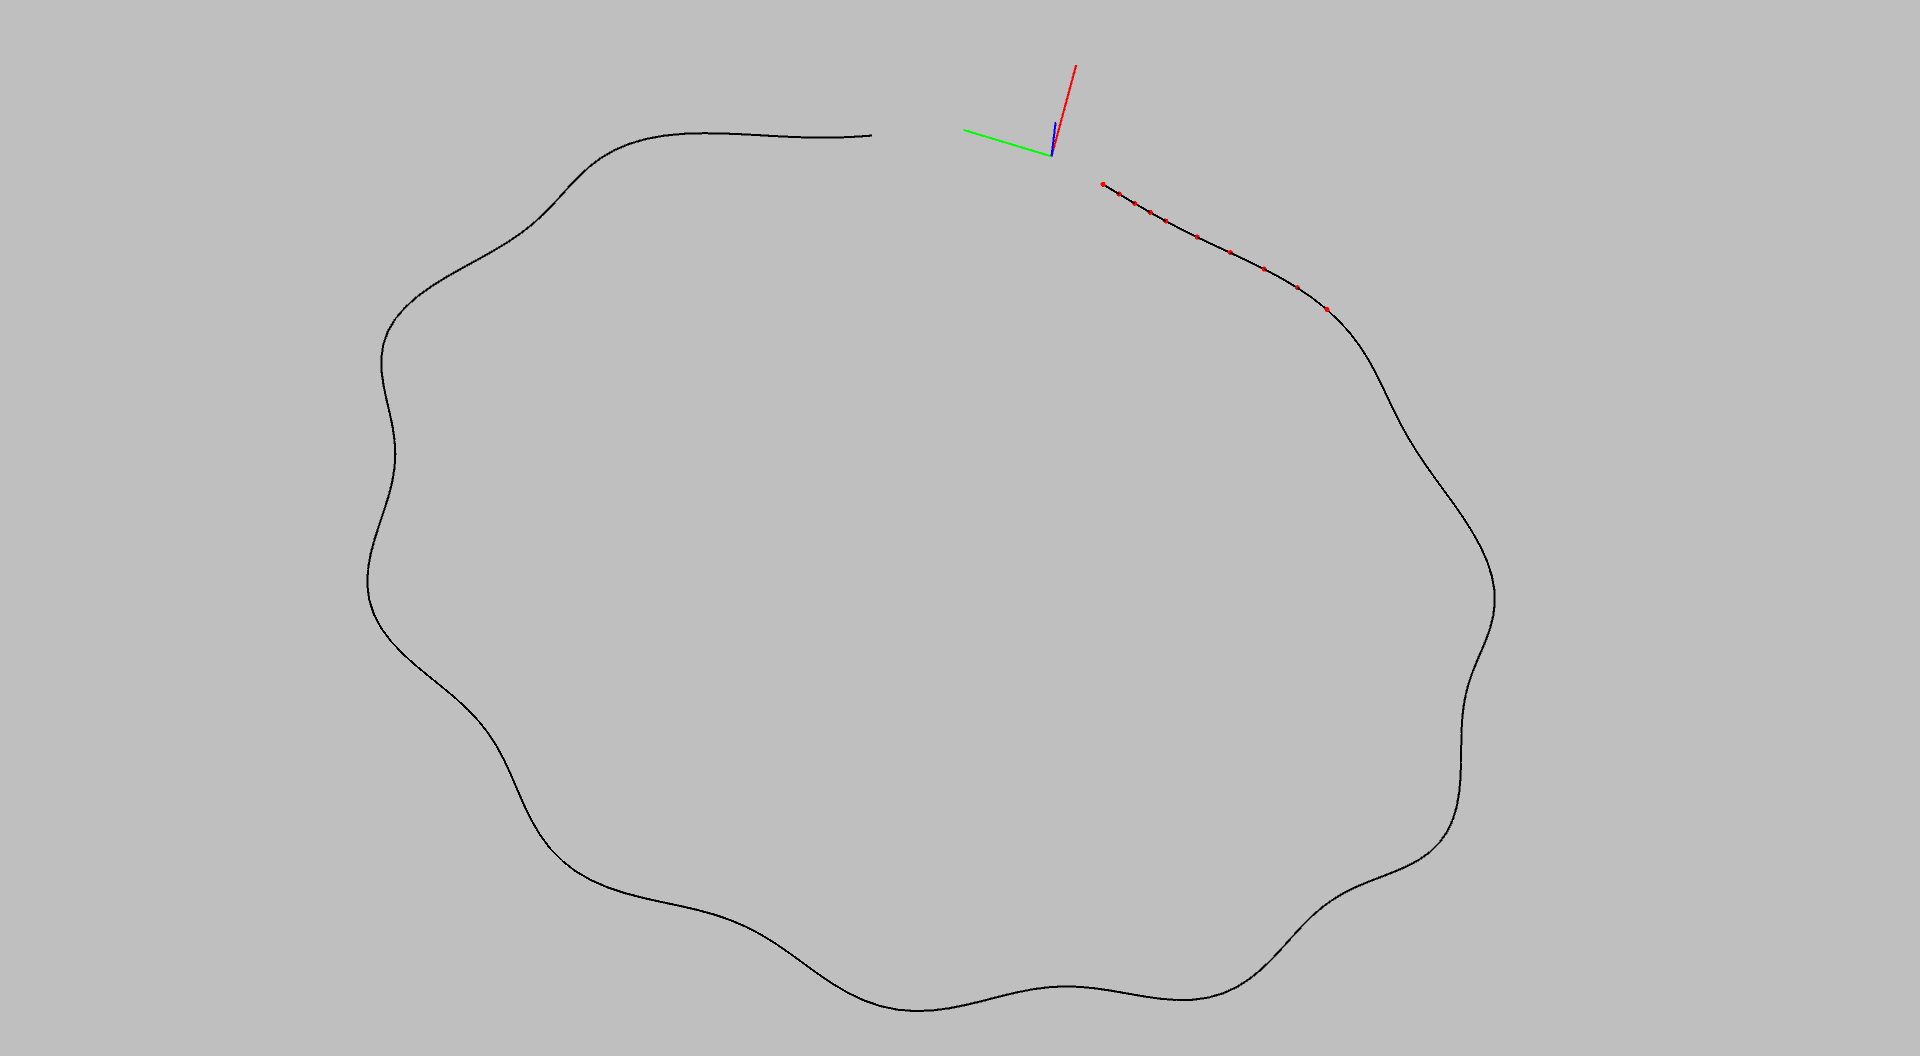
\includegraphics[width=15cm]{images/trajectory.png}
\end{figure} 

\newpage
\item 仿真数据集有噪声(不同噪声设定时,需要配置 vins 中 imu noise 大小)

\begin{itemize}
  \item with IMU noise01
  
  \begin{lstlisting}
  acc_n: 0.019
  gyr_n: 0.015
  acc_w: 0.0001
  gyr_w: 1.0e-5
  \end{lstlisting}

  \begin{figure}[htbp] 
	\centering
	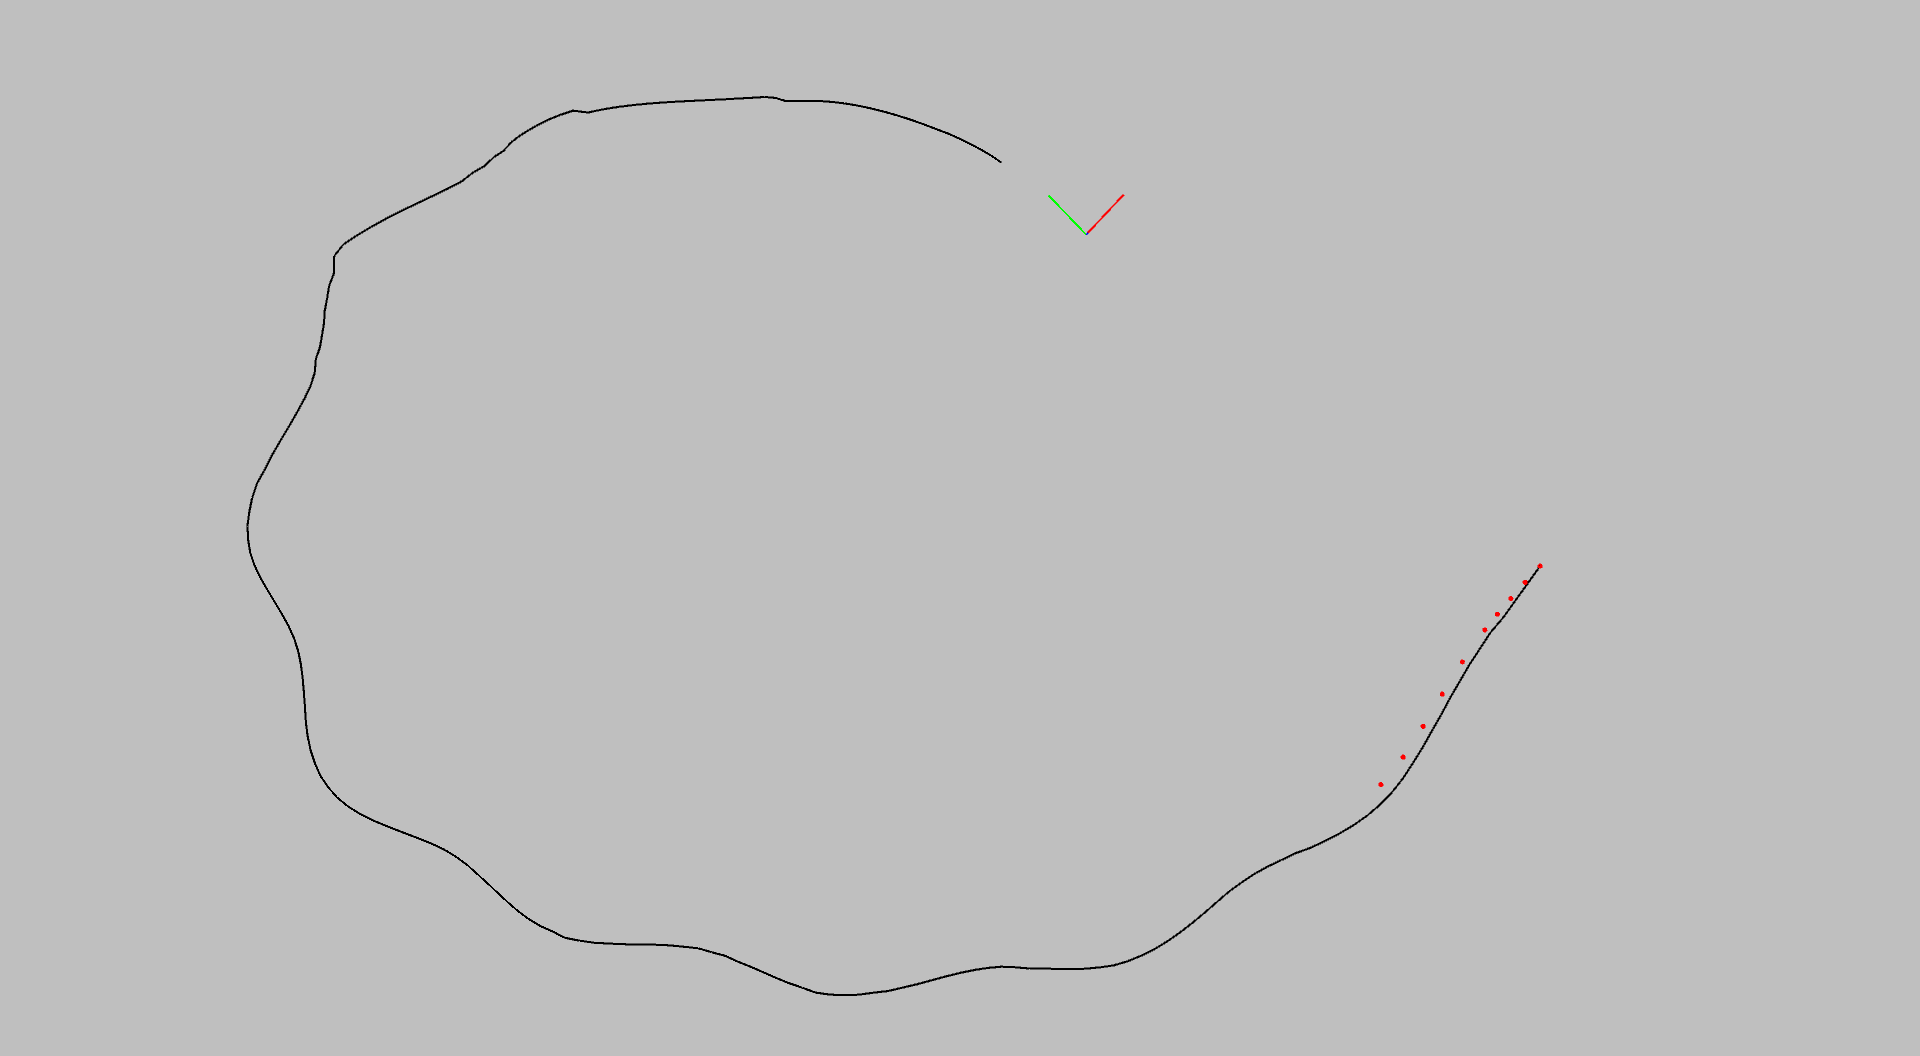
\includegraphics[width=15cm]{images/trajectory_noise01.png}
  \end{figure} 
  
  \item with IMU noise02
  
  \begin{lstlisting}
  acc_n: 0.019
  gyr_n: 0.0005
  acc_w: 0.0001
  gyr_w: 1.0e-6
  \end{lstlisting}
  
  \begin{figure}[htbp] 
	\centering
	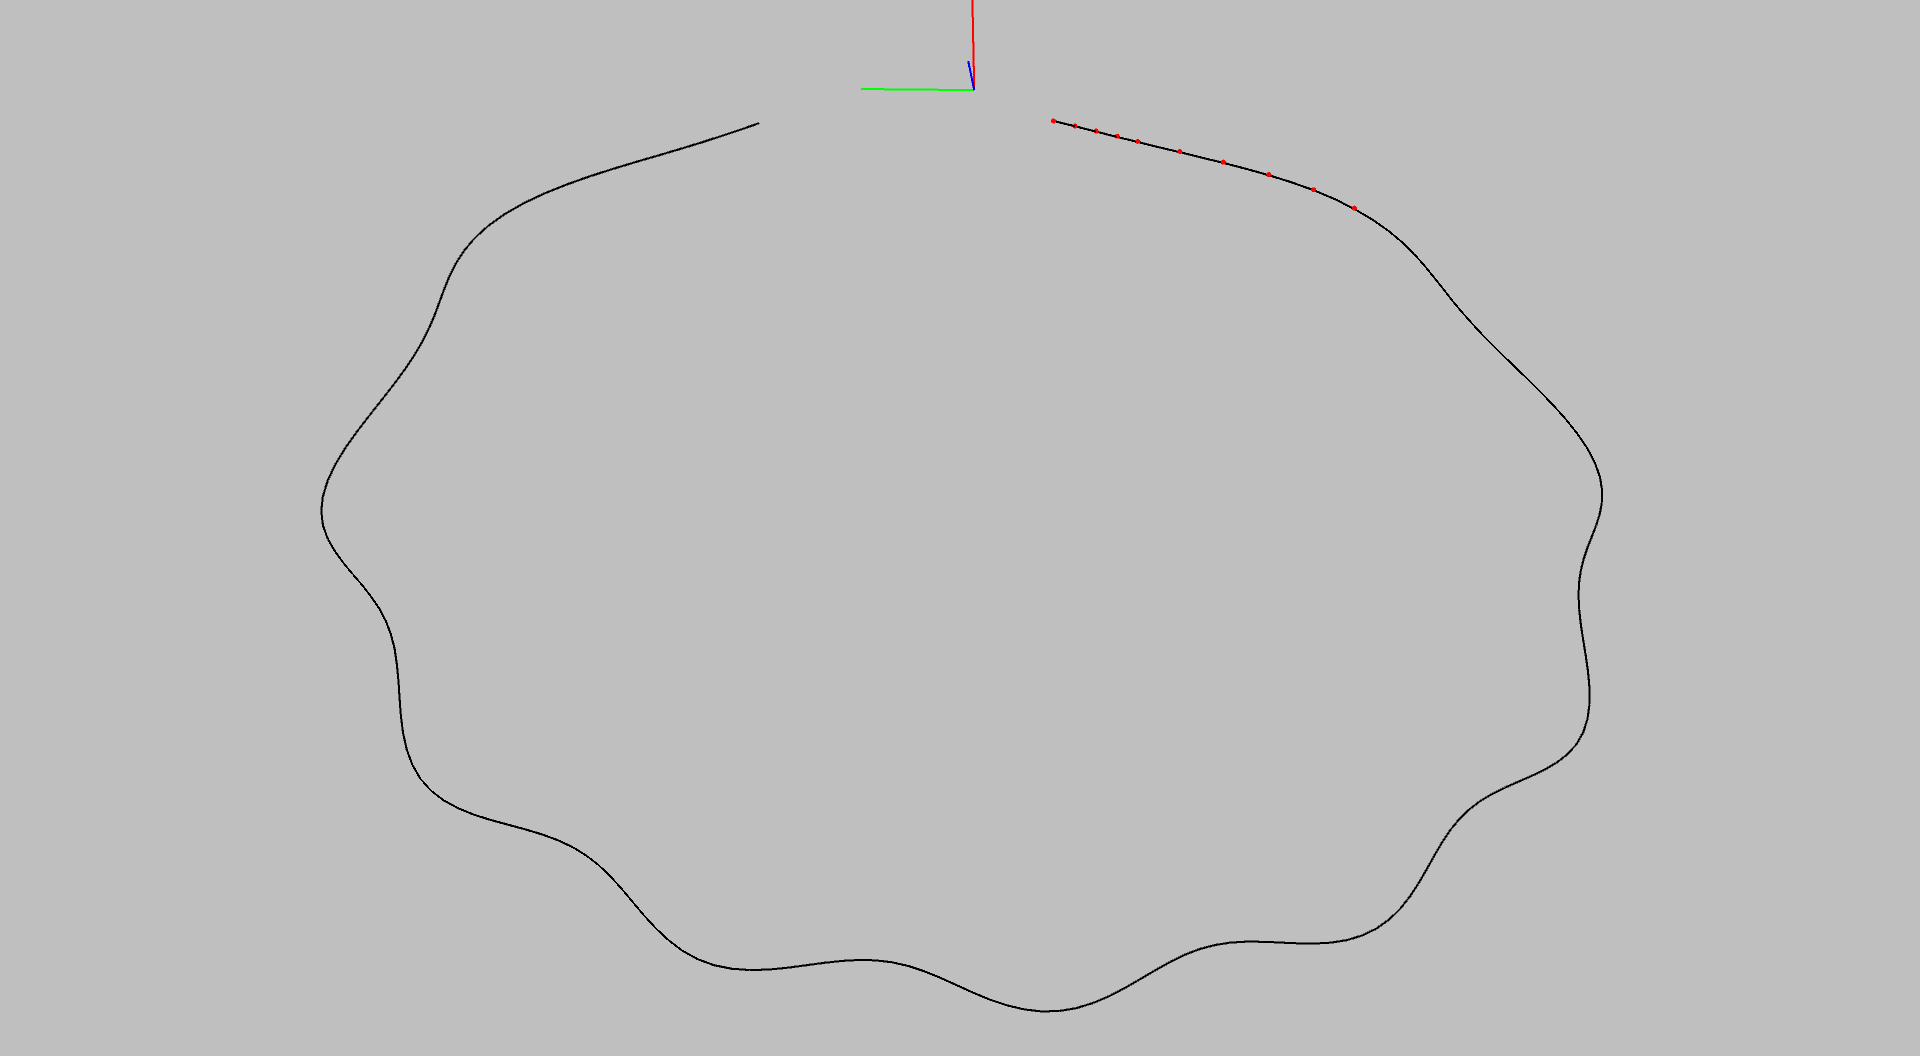
\includegraphics[width=15cm]{images/trajectory_noise02.png}
  \end{figure} 

\end{itemize}


\end{enumerate}


\end{document}

